% !TeX root = ../presentation.tex

\section*{Introducción}
%----------------------------------------------------------------------------------
\begin{frame}{{Antecedentes}}

    \begin{alertblock}{Metasuperficies plasmónicas para biosensado}
        \begin{itemize}%[<+->]
         \itemsep9pt
         \item Arreglos bidimensionales de \textbf{nanoestructuras metálicas} (meta-átomos) soportadas por un sustrato.$^1$
        \end{itemize}
    \end{alertblock}
    
    \begin{center}
  	\begin{tikzpicture}[node distance=1em and 1em,font=\small]
        \path (0,0) node [flowbox] (bio) {\fbtitle{Meta-átomos}\vphantom{yÖ}
	    \nodepart{two}
         \begin{minipage}{.25\textwidth} \begin{itemize}
			\item Geometría
			\item Material
			\item Distribución
               \begin{itemize}
                  \item Desordenada $^{4,5}$
                  \item Periódica $^{2,3}$
               \end{itemize}
            \item \textbf{Perfecto soporte sobre sustrato}
         \end{itemize}\end{minipage}
        };

        \node[flowbox, below = of bio] (exp) {\fbtitle{Respuesta óptica}\vphantom{yÖ}
        \nodepart{two}
         \begin{minipage}{.25\textwidth} \begin{itemize}
            \item Resultados experimentales$^{2,3,4,5}$
            \item Simulaciones numéricas$^{2,3,4}$
            \item Teorías de medio efectivo$^5$
         \end{itemize}\end{minipage}
        };

        \node at (7,-1){\includegraphics[scale = .6]{background.png}};

        \node[draw,circle,inner sep=0.5pt, font=\tiny] at (2.85, 1) {A};
%         \node at (2.85, 1) {\ding{173}}; %2

        \node[draw,circle,inner sep=0.5pt, font=\tiny] at (5.8,1.2) {B};
%         \node at (5.8,1.2) {\ding{174}};   %3

        \node[draw,circle,inner sep=0.5pt, font=\tiny] at (6,-1.5) {C};
%         \node at (6,-1.5) {\ding{175}}; %4

        \node[draw,circle,inner sep=0.5pt, font=\tiny] at (9.6,1) {D};
%         \node at (9.6,1) {\ding{176}}; %5
    \end{tikzpicture}
    \end{center}   
    
    \vspace*{-4em}
    \begin{columns}
        \column{.35\textwidth}
        \column{.65\textwidth}
        \noindent\rule{.25\textwidth}{0.4pt}	
         \begin{spacing}{0}\fontsize{4}{5} \selectfont
            $^{\text{\;\;\;\;\;}1}$ \fullcite{gonzalez-alcalde_large_2020}\\
            $^{2\text{, A}}$ \fullcite{feuz_improving_2010}\\
            $^{3\text{, B}}$ \fullcite{kabashin_plasmonic_2009}\\
            $^{4\text{, C}}$ \fullcite{qiu_dual_2020}\\
            $^{5\text{, D}}$ \fullcite{svedendahl_refractometric_2014}
         \end{spacing}	
   \end{columns}
\end{frame}

% %----------------------------------------------------------------------------------
% \begin{frame}{{Objetivo}}
% \begin{columns}
%    \column{.55\textwidth}
%    \begin{alertblock}{Incrustamiento parcial de meta-átomos en el sustrato}
%         \begin{itemize}%[<+->]
%          \item Resultados del proceso de fabricación$^1$
%          \item Característica deseable para metasupeficies enfocadas para biosensado (Acoplamiento con sistemas de microfluídica)
%          \item ¿Cuál es su efecto en la respuesta óptica?
%         \end{itemize}
%     \end{alertblock}
%    \column{.45\textwidth}
%
%    \begin{center}
%   	\begin{tikzpicture}[node distance=1em and 1em,font=\small]
%         \path (0,0) node [flowbox] (bio) {\fbtitle{Sistema de estudio}\vphantom{yÖ}
% 	    \nodepart{two}
%          \begin{minipage}{.95\textwidth}
%          Nanopartíula esférica apta para biosensado en metasuperficies\\
%
%          \begin{itemize}
% 			\item Meta-átomo: 12.5 nm AuNP
% 			\item Matriz: Aire
% 			\item Sustrato: Vidrio
%          \end{itemize}\end{minipage}
%         };
%     \end{tikzpicture}
%     \end{center}
% \end{columns}
%
%     \begin{center}
%   	\begin{tikzpicture}[node distance=1em and 1em,font=\small]
%         \node at (0,0) {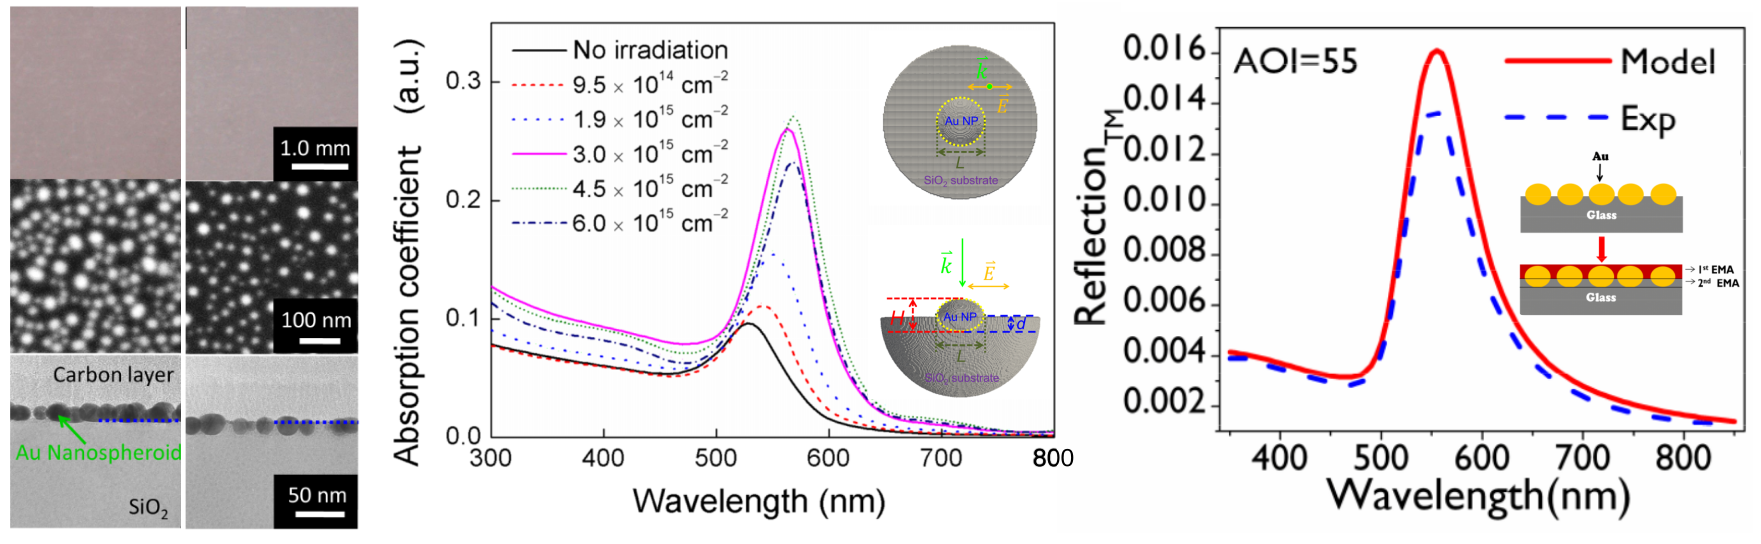
\includegraphics[scale = .7]{embedding.png}};
%
%         \node at (-5.35,1.45) {\ding{172}}; %1
%         \node at (1.25,1.35) {\ding{173}};   %2
%     \end{tikzpicture}
%     \end{center}
%
%     \vspace*{0em}
%         \noindent\rule{.25\textwidth}{0.4pt}
%          \begin{spacing}{0}\fontsize{4}{12} \selectfont
%             $^1$ \fullcite{meng_anisotropic_2015}\\
%             $^2$ \fullcite{moirangthem_enhanced_2012}
%          \end{spacing}
% \end{frame}


%----------------------------------------------------------------------------------
\begin{frame}{Objetivo}{Estudio del incrustamiento parcial de meta-átomos en el sustrato}
   \begin{center}
  	\begin{tikzpicture}[node distance=1em and 1em,font=\small]
        \path (-7.5,0) node [flowbox] (bio) {\fbtitle{Incrustamiento de meta-átomos}\vphantom{yÖ}
	    \nodepart{two}
         \begin{minipage}{.3\textwidth}
         \begin{itemize}%[<+->]
         \item Proceso de fabricación$^1$
         \item Característica deseable para biosensado
            \begin{itemize}
            \item Acoplamiento con  sistemas de microfluídica$^2$
            \end{itemize}
         \item \textbf{¿Detección óptica?}
        \end{itemize}\end{minipage}
        };
%
         \node at (0,-1.5) {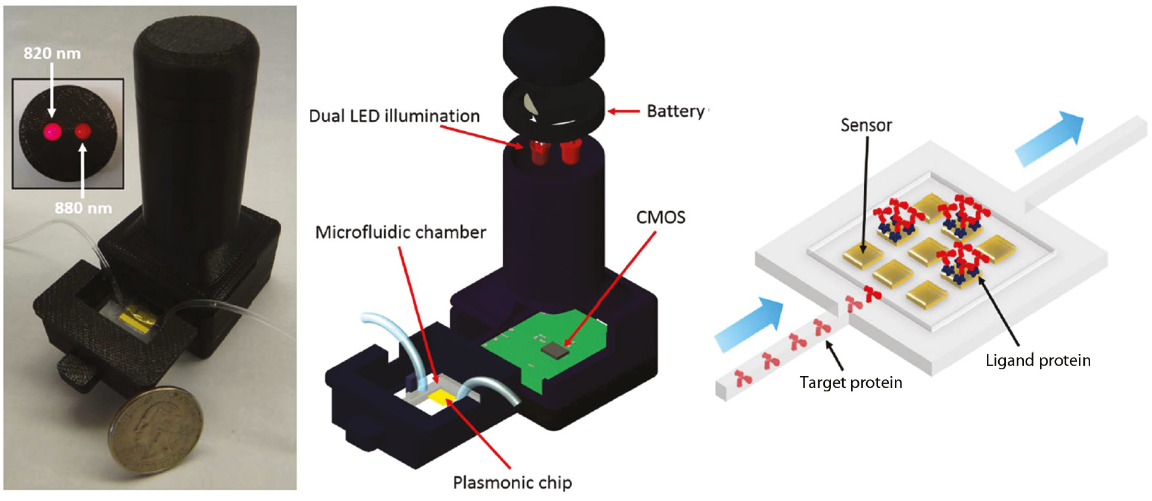
\includegraphics[scale = .3, trim = {0 0 0 0}, clip]{micro.png}};
         \node at (0,+1.5) {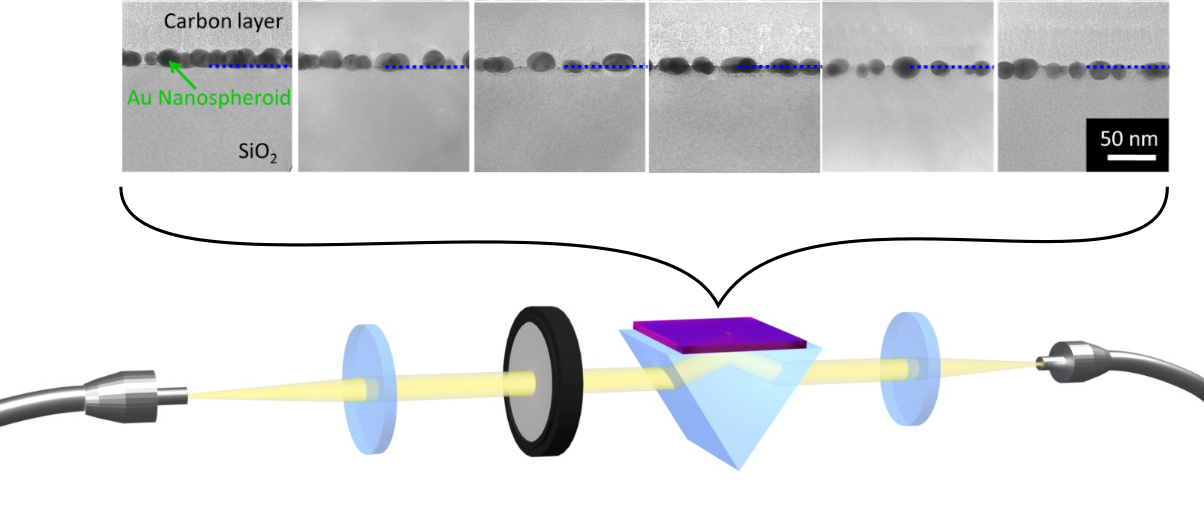
\includegraphics[scale = 1.05, trim = {30 80 10 0}, clip]{exp-NPs.png}};

         \node[draw,circle,inner sep=0.5pt, font=\tiny] at (-4.85,2.25) {A};
         \node[draw,circle,inner sep=0.5pt, font=\tiny] at (-4.85,.45) {B};
    \end{tikzpicture}
\end{center}

    \vspace*{0em}
        \noindent\rule{.25\textwidth}{0.4pt}
         \begin{spacing}{0}\fontsize{4}{12} \selectfont
            $^{1\text{, A}}$ \fullcite{meng_anisotropic_2015}\\
            $^{2\text{, B}}$ \fullcite{lopez_recent_2017}
         \end{spacing}
\end{frame}


%----------------------------------------------------------------------------------
\begin{frame}{Sistema de interés}{Meta-átomo: Nanopartícula (NP) esférica de oro (Au) apta para biosensado}

      \begin{center}
  	\begin{tikzpicture}[node distance=1em and 1em,font=\small]
        \path (-7.5,-1.25) node [flowbox] (bio) {\fbtitle{FC-UNAM$^1$ -- INAOE$^{2}$}\vphantom{yÖ}
	    \nodepart{two}
         \begin{minipage}{.35\textwidth}
          Desarrollo de un biosensor plasmónico:\\

          \begin{itemize}
            \item Colaboración teórico-experimental
			\item Metasuperficie desordenada
            \item Mediciones de reflectancia
%                \begin{itemize}
%                   \item Polarización $s$
%                   \item Polarización $p$
%                \end{itemize}
% 			\item Incidencia oblicua
         \end{itemize}\end{minipage}
        };

        \node at (-2.25,-0.25) {Esquema del sistema experimental$^3$:};
          \node at (0,-1.75) {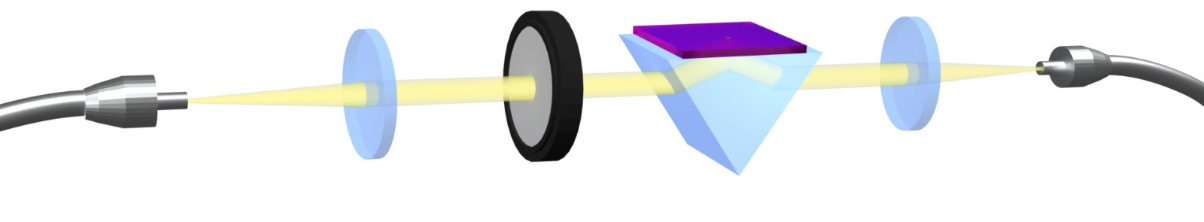
\includegraphics[scale = .8]{sistExp.png}};

        \node at (-3,-0.75) {\footnotesize Fuente de luz blanca};
        \node at (1.,-0.75) {\footnotesize Muestra sobre prisma};
        \node at (3.5,-0.75) {\footnotesize Detector};

        \node at (-1.6,-2.5) {\footnotesize Lente};
        \node at (-.25,-2.5) {\footnotesize Polarizador};
        \node at (2.1,-2.5) {\footnotesize Lente};

        \path (-7.5,-4.25) node [flowbox] (bio) {\fbtitle{Meta-átomo:}\vphantom{yÖ}
	    \nodepart{two}
         \begin{minipage}{.25\textwidth}
          \begin{itemize}
			\item AuNP esférica
            \item Radio $a$: 12.5 nm
			\item Matriz: Aire
			\item Sustrato: Vidrio
			\item Incrustamiento parcial
         \end{itemize}\end{minipage}
        };

        \node at (0,-5) {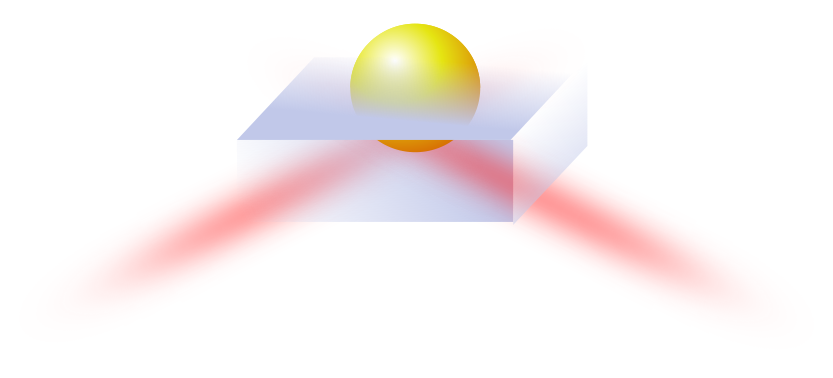
\includegraphics[scale = 1.1]{NP.png}};
        \node at (-3,-3.25) {Esquema del meta-átomo:};

        \node at (1,-3.75) {\footnotesize Matriz};
        \node at (.5,-5) {\footnotesize Sustrato};

    \end{tikzpicture}
    \end{center}

    \vspace*{-3.5em}
        \noindent\rule{.25\textwidth}{0.4pt}
         \begin{spacing}{0}\fontsize{4}{12} \selectfont
            $^1$ Grupo de Nanoplasmónica\\
            $^2$ Grupo de Biofotónica y Grupo de Optoelectrónica de semiconductores orgánicos e híbridos\\
            $^3$ Esquema realizado Juan Pablo Cuanalo Fernández.
         \end{spacing}
\end{frame}
